\epi{我对外科手术般进入我的身体总是有恐惧。你知道我说的是什么。}{\textit{eXistenZ}\\\textsc{TED PIKUL}}
\noindent{}
\gomarginpar{下面的内容来自 \cite{go_interfaces}。是 Ian Lance Taylor 编写的,他是 Go 的作者之一。}
在 Go 中,保留字 \first{\emph{interface}}{interface} 被赋予了多种不同的含义。
每个类型都有接口,意味着对那个类型\emph{定义了方法集合}
\index{interface!set of methods}。这段代码定义了具有一个字段和两个方法的结构类型 \type{S}。
\begin{lstlisting}[caption=定义结构和结构的方法,label=src:interface object]
type S struct { i int }
func (p *S) Get() int { return p.i }
func (p *S) Put(v int) { p.i = v }
\end{lstlisting}
也可以定义\first{接口类型}{interface!type},仅仅是方法的集合。
这里定义了一个有两个方法的接口 \type{I}:
\begin{lstlisting}
type I interface {
  Get() int
  Put(int)
}
\end{lstlisting}
\begin{lbar}
接口类型就是方法的集合。
\end{lbar}

\noindent对于接口 \type{I},\type{S} 是合法的\emph{实现},因为它定义了 \type{I}
所需的两个方法。注意,即便是没有明确定义 \type{S} 实现了 \type{I},这也是正确的。

Go 程序可以利用这个特点来实现接口的另一个含义,就是
\first{接口值}{interface!value}:

\begin{lstlisting}
func f(p I) {  |\longremark{定义一个函数接受一个接口类型作为参数;}|
    fmt.Println(p.Get()) |\longremark{\var{p} 实现了接口 \type{I},\emph{必须}有 \func{Get()} 方法;}|
    p.Put(1) |\longremark{\func{Put()} 方法是类似的。}|
}
\end{lstlisting}
\showremarks
这里的变量 \var{p} 保存了接口类型的值。因为
\type{S} 实现了 \type{I},可以调用 \func{f} 向其传递 \type{S} 类型的值的指针:
\begin{lstlisting}
var s S; f(&s)
\end{lstlisting}

获取 \type{s} 的地址,而不是 \type{S} 的值的原因,是因为在 \type{s} 
的指针上定义了方法,参阅上面的代码 \ref{src:interface object}。
这并不是必须的——可以定义让方法接受值——但是这样的话 \func{Put} 方法就不会像期望的那样工作了。

The fact that you do not need to declare whether or not a type implements an
interface means that Go implements a form of 
\first{duck typing}{duck typing}\cite{duck_typing}. 
This is not
pure duck typing, because when possible the Go compiler will statically
check whether the type implements the interface. However, Go does have a
purely dynamic aspect, in that you can convert from one interface type
to another. In the general case, that conversion is checked at runtime.
If the conversion is invalid --- if the type of the value stored in the
existing interface value does not satisfy the interface to which it is
being converted --- the program will fail with a runtime error.

Interfaces in Go are similar to ideas in several other programming languages:
pure abstract virtual base classes in C++, typeclasses in Haskell or duck typing
in Python. However there is no other language which combines
interface values, static type checking, dynamic runtime conversion, and no
requirement for explicitly declaring that a type satisfies an interface. The
result in Go is powerful, flexible, efficient, and easy to write.

\subsection{Which is what?}
Lets define another type that also implements the interface \type{I}:
\begin{lstlisting}[caption=Another type that implements I]
type R struct { i int }
func (p *R) Get() int { return p.i }
func (p *R) Put(v int) { p.i = v }
\end{lstlisting}
The function \func{f} can now accept variables of type \type{R} and \type{S}.
Suppose you need to know the actual type in the function \func{f}. In Go you can 
figure that out by using a \first{type switch}{type switch}.

\begin{lstlisting}
func f(p I) {
    switch t := p.(type) { |\longremark{The type switch. Use \key{(type)} in a \key{switch} %
statement. We store the type in the variable \var{t};}|
        case *S: |\longremark{The actual type of \var{p} is a pointer to \type{S};}|
        case *R: |\longremark{The actual type of \var{p} is a pointer to \type{R};}|
        case S:  |\longremark{The actual type of \var{p} is a \type{S};}|
        case R:  |\longremark{The actual type of \var{p} is a \type{R};}|
        default: |\longremark{It's another type that implements \type{I}.}|
    }
}
\end{lstlisting}
\showremarks
Note that a type switch is the only way to figure out what type of an interface variable is. Using
\key{(type)} outside a \key{switch} is illegal.

\subsection{Empty interface}
Since every type satisfies the empty interface:
\type{interface\{\}}. We can create a generic function which 
has an empty interface as its argument:
\begin{lstlisting}[caption=A function with a empty interface argument,label=src:interface empty]
func g(any interface{}) int { 
    return any.(I).Get() 
}
\end{lstlisting}
The \lstinline{return any.(I).Get()} is the tricky bit in this function.
The value \var{any} has type \type{interface\{\}}, meaning no guarantee
of any methods at all: it could contain any type. The \lstinline{.(I)}
is a \first{type assertion}{type assertion} which converts \var{any} to an interface of
type \type{I}. If we have that type we can invoke the \func{Get()}
function.
So if we create a new variable of the type \type{*S}, we can just
call \func{g()}, because \type{*S} also implements the empty interface.
\begin{lstlisting}
s = new(S)
fmt.Println(g(s));
\end{lstlisting}
The call to \func{g} will work fine and will print 0. If we however
invoke \func{g()} with a value that does not implement \type{I} we have
a problem:
\begin{lstlisting}[caption=Failing to implement an interface,label=src:interface fail]
i := 5		|\coderemark{Make i a "lousy" \texttt{int}}|
fmt.Println(g(i))
\end{lstlisting}
This compiles OK, but when we run this we get slammed with:

\noindent\error{panic: interface conversion: int is not main.I: missing
method Get}

\noindent{}Which is completely true, the built-in type \type{int} does not
have a \func{Get()} method.

\subsection{Checking for interfaces}
In your code you want to prevent these kind of errors, therefor Go provides you 
with a way to check if a variable implements a certain interface, again this 
uses a type assertion, but now in an \key{if} statement.

\begin{lstlisting}
if ok := any.(I); ok { 
   /* any implements the interface I */
} 
\end{lstlisting}

\section{Methods}
Methods are functions that have an receiver (see chapter
\ref{chap:functions}).
You can define methods on any type (except on non-local types, this includes
built-in types: the type \type{int} can not have methods).
You can however make a new integer type with its own methods. For example:
\begin{lstlisting}
type Foo int

func (self Foo) Emit() {
  fmt.Printf("%v", self)
}

type Emitter interface {
  Emit()
}
\end{lstlisting}
Doing this on non-local (types defined in other packages) types yields:
% Empty line here is critical, otherwise no new paragraph is created

\begin{minipage}{.5\textwidth}
\begin{lstlisting}[linewidth=.7\textwidth,caption=Failure extending built-in types]
func (i int) Emit() {
  fmt.Printf("%d", i)
}
\end{lstlisting}
\noindent\error{cannot define new methods\\ on non-local type int}
\end{minipage}
\begin{minipage}{.5\textwidth}
\begin{lstlisting}[caption=Failure extending non-local types]
func (a *net.AddrError) Emit() {
  fmt.Printf("%v", a)
}
\end{lstlisting}
\noindent\error{cannot define new methods\\ on non-local type net.AddrError}
\end{minipage}

\paragraph{}  %% needed otherwise the minipage flows over

\subsection{Methods on interface types}
An interfaces defines a set of methods. A method contains the actual code.
In other words, an interface is the definition and the methods are the implementation.
So a receiver can not be a defined for interface
types, doing so results in a \error{invalid receiver type ...} compiler
error. The authoritative word from the language spec \cite{go_spec}:
\begin{quote}
The receiver type must be of the form \type{T} or \type{*T} where
\type{T} is a type name. \type{T} is called the receiver base type or just base 
type. The base type must
not be a pointer or interface type and must be declared in the same
package as the method.
\end{quote}

\subsection{Pointers to interfaces}
Creating a pointer to an interface value is a useless action in Go.
\todo{Interfaces is not a pointer, not reference type}
\gomarginpar{Go \gorelease{2010-10-13}.} It is in fact illegal to
create a pointer to an interface value. The release notes for that release that
made them illegal leave no room for doubt:
\begin{quote}
The language change is that uses of pointers to interface values no longer 
automatically dereference the pointer.  A pointer to an interface value is more 
often a beginner's bug than correct code.
\end{quote}
From the \cite{go_faq}.  If not for this restriction, this code:
\begin{lstlisting}
var buf bytes.Buffer
io.Copy(buf, os.Stdin)
\end{lstlisting}
Would copy standard input into a copy of \var{buf}, not into \var{buf} itself. 
This is almost never the desired behavior.

\section{Interface names}
By convention, one-method interfaces are named by the method name plus
the \emph{-er} suffix: Read\emph{er}, Writ\emph{er}, Formatt\emph{er} etc.

There are a number of such names and it's productive to honor them and
the function names they capture. \func{Read}, \func{Write},
\func{Close}, \func{Flush}, \func{String} and
so on have canonical signatures and meanings. To avoid confusion, don't
give your method one of those names unless it has the same signature and
meaning. Conversely, if your type implements a method with the same
meaning as a method on a well-known type, give it the same name and
signature; call your string-converter method \func{String} not
\func{ToString}.
\gomarginpar{Text copied from \cite{effective_go}.}

\section{A sorting example}
\label{sec:a sorting example}
Recall the Bubblesort exercise (Q\ref{ex:bubble}), where we sorted an
array of integers:
\begin{lstlisting}
func bubblesort(n []int) {
    for i := 0; i < len(n)-1; i++ {
	for j := i + 1; j < len(n); j++ {
	    if n[j] < n[i] {
		    n[i], n[j] = n[j], n[i]
	    }
	}
    }
}
\end{lstlisting}
A version that sorts strings is identical except for the signature of
the function:
\begin{lstlisting}
func bubblesortString(n []string) { /* ... */ }
\end{lstlisting}
Using this apprach would lead to two functions, one for each type. By using
interfaces we can make this more \index{generic} generic.

Lets create a new function that will sort both strings and
integers, something along the lines of this non-working example:
\begin{lstlisting}
func sort(i []interface{}) { |\longremark{Our function will receive a slice of %
empty interfaces;}|
    switch i.(type) {        |\longremark{Using a type switch we find out what the %
actual type is of the input;}|
	case string:         |\longremark{And then sort accordingly;}|
	    // ...
	case int:
	    // ...
    }
    |\longremark{Return the sorted slice.}|
}
\end{lstlisting}
\showremarks
But when we call this function with \lstinline|sort([]int{1, 4, 5})|, it
fails with:
\error{cannot use i (type []int) as type []interface { } in function argument}

This is because Go can not easily convert to a \emph{slice} of interfaces.
Just converting to an interface is easy, but to a slice is much more costly.
To keep a 
\gomarginpar{The full mailing list discussion on this subject
can be found at \cite{go_nuts_interfaces}.}
long story short: Go does not (implicitly) convert slices for you.

So what is the Go way of creating such a "generic" function? 
Instead of doing the type inference our selves with a type switch, we let
Go do it implicitly:
The following steps are required:
\begin{enumerate}
\item Define an interface type (called \type{Sorter} here) with a number of 
methods needed for sorting.
We will at least need a function to get the length of the slice,
a function to compare two values and a swap function;
\begin{lstlisting}
type Sorter interface {
    Len() int           |\coderemark{\texttt{len()} as a method}|
    Less(i, j int) bool |\coderemark{\texttt{p[j] $<$ p[i]} as a method}|
    Swap(i, j int)      |\coderemark{\texttt{p[i], p[j] = p[j], p[i]} as a method}|
}
\end{lstlisting}
\item Define new types for the slices we want to sort. Note that we
declare slice types;
\begin{lstlisting}
type Xi []int
type Xs []string
\end{lstlisting}
\item Implementation of the methods of the \type{Sorter} interface.
For integers:
\begin{lstlisting}
func (p Xi) Len() int               { return len(p) }
func (p Xi) Less(i int, j int) bool { return p[j] < p[i] }
func (p Xi) Swap(i int, j int)      { p[i], p[j] = p[j], p[i] }
\end{lstlisting}
And for strings:
\begin{lstlisting}
func (p Xs) Len() int               { return len(p) }
func (p Xs) Less(i int, j int) bool { return p[j] < p[i] }
func (p Xs) Swap(i int, j int)      { p[i], p[j] = p[j], p[i] }
\end{lstlisting}
\item Write a \emph{generic} Sort function that works on the \type{Sorter} interface.
\begin{lstlisting}
func Sort(x Sorter) { |\longremark{\var{x} is now of the \texttt{Sorter} type;}|
    for i := 0; i < x.Len() - 1; i++ { |\longremark{Using the defined functions, we implement Bubblesort.}|
	for j := i + 1; j < x.Len(); j++ {
	    if x.Less(i, j) {
		x.Swap(i, j)
	    }
	}
    }
}
\end{lstlisting}
\showremarks
\end{enumerate}
We can now use you generic \func{Sort} function as follows:
\begin{lstlisting}
ints := Xi{44, 67, 3, 17, 89, 10, 73, 9, 14, 8}
strings := Xs{"nut", "ape", "elephant", "zoo", "go"}

Sort(ints)
fmt.Printf("%v\n", ints)
Sort(strings)
fmt.Printf("%v\n", strings)
\end{lstlisting}

\section{Introspection}
\label{sec:introspection}
In a program, you can discover the dynamic type of an interface variable
by using a \key{switch}.
Such a type assertion\gomarginindex{Type assertion.}{type assertion} uses
the syntax of a type assertion with the keyword \key{type} inside the
parentheses. If the switch declares a variable in the expression, the
variable will have the corresponding type in each clause.
\begin{lstlisting}[caption=Dynamically find out the type]
package main
type PersonAge struct { |\longremark{First we define two structures as a new type, %
\texttt{PersonAge};}|
	name string
	age  int
}

type PersonShoe struct { |\longremark{And \texttt{PersonShoe};}|
	name     string
	shoesize int
}

func main() {
	p1 := new(PersonAge)
	p2 := new(PersonShoe)
	WhichOne(p1)
	WhichOne(p2)
}

func WhichOne(x interface{}) { |\longremark{This function must accept \emph{both} %
types as valid input, so we use the empty Interface, which every type implements;}|
	switch t := x.(type) { |\longremark{The type switch: \texttt{(type)};}|
	case *PersonAge:	|\longremark{When allocated with \func{new}, it's a %
pointer. So we check for \type{*PersonAge}. If \func{WhichOne()} was %
called with a non pointer value, we should check for \type{PersonAge}.}|
		println("Age person")
	case *PersonShoe:
		println("Shoe person")
	}
}
\end{lstlisting}
\showremarks

The following is another example of performing a type switch, but this
time checking for more (built-in) types:
\begin{lstlisting}[caption=A more generic type switch]
switch t := interfaceValue.(type) { |\coderemark{The type switch}|
case bool:
    fmt.Printf("boolean %t\n", t)
case int:
    fmt.Printf("integer %d\n", t)
case *bool:
    fmt.Printf("pointer to boolean %t\n", *t)
case *int:
    fmt.Printf("pointer to integer %d\n", *t)
default:
    fmt.Printf("unexpected type %T", t)  // \%T prints type
}
\end{lstlisting}

\subsection{Introspection and reflection}
\label{subsec:introspection and reflection}
In the following example we want to look at the "tag" (here named
"namestr") defined in the
type definition of \type{Person}. To do this we need the
\package{reflect}\index{package!reflect} package (there is no other way in Go). Keep in mind
that looking at a tag means going back the \emph{type} definition. So
we use the \package{reflect} package to figure out the type of the variable
and \emph{then} access the tag.

\begin{lstlisting}[caption=使用反射自省,label=src:introspection]
|\begin{tikzpicture}[overlay]
\ubrace{3.2,-5.2}{2.2,-5.2}{%
We are dealing with a \type{PtrValue} and according %
to the documentation\footnote{\texttt{godoc reflect}}:%
\begin{quote} %
Elem 返回 v 指向的值。%
如果 v 是空指针,Elem 返回空值。%
\end{quote} %
同样的在 \var{t} 使用 \func{Elem()} 得到了指针指向的值。}
%%We can use \func{Elem()} to get the type the pointer points to. %
%%In this case \type{*reflect.StructValue}. We have also %
%%used \type{reflect.NewValue(i)} for the type assertion, so that %
%%we get back types in the \type{*reflect} namespace;}
%
\ubrace{4.3,-5.2}{3.6,-5.2}{在 \var{Value} 使用函数 \func{Type()} %
返回 \type{reflect.Type}。需要获取类型的原因是因为那是标签定义的地方;}%
%
\ubrace{7.7,-5.2}{4.8,-5.2}{%
这样获得了 \var{reflect.Type}:\\%
\begin{quote} %
\ldots 返回接口类型 \type{Type} 的对象。包含了指向 \type{*StructType}、\type{*IntType}等类型结构的指针。%
描述了底层类型的细节信息。type switch 或者类型断言可以展示的。%
\end{quote} %
因此可以访问结构中特殊类型的成员。通过 \type{(*reflect.StructType)} 实现;}
%
\ubrace{8.9,-5.2}{7.9,-5.2}{%
\type{StructType} 有若干方法,其中一个是 \func{Field($n$)},返回结构的第 $n^{th}$ 个字段。%
这个返回的类型是 \type{StructField};}
%
\ubrace{9.6,-5.2}{9.1,-5.2}{%
结构 \type{StructField} 有成员 \var{Tag},返回字符串类型的标签名。%
因此,在第 $0^{th}$ 个字段上可以用 \func{.Tag} 访问这个名字:\texttt{Field(0).Tag}。%
这\emph{最终}给出\texttt{namestr}。}
\end{tikzpicture}|
type Person struct {
    name string "namestr" |\coderemark{\texttt{"namestr"} 是标签}|
    age  int
}

p1 := new(Person)   |\coderemark{\func{new} 返回 Person 的指针}|
ShowTag(p1)	    |\coderemark{调用 \func{ShowTag()} 并传递指针}|

func ShowTag(i interface{}) {
 switch t := reflect.NewValue(i).(type) { |\coderemark{在 \type{reflect} 值上的类型断言}|
 case *reflect.PtrValue:	  |\coderemark{因此是 \var{*reflect.PtrValue}}|
	tag := t.Elem().Type().(||*reflect.StructType).Field(0).Tag
||
\end{lstlisting}
Elem 返回 v 指向的值。%
如果 v 是空指针,Elem 返回空值。%

\showremarks

%% look at layout
To make the difference between looking a types and values more clear,
that a look at the following code:
\begin{lstlisting}[caption=Reflection and the type and value]
func show(i interface{}) {
    switch t := i.(type) {
      case *Person:
        r := reflect.NewValue(i) |\coderemark{Enter the world of reflection}|
	tag := |\longremark{Here we want to get the "tag", which means %
going for the type. Thus we need\newline\lstinline{Elem().Type().(*reflect.StructType)} to get to it;}|
	  r.(*reflect.PtrValue).Elem().Type().(*reflect.StructType).Field(0).tag
	nam := |\longremark{Now we want to get access to the %
\emph{value} of one of the members and we %
employ\newline\lstinline{Elem().(*reflect.StructValue)} to get to it. %
Now we have arrived at the structure. Then we go the the first field %
\lstinline{Field(0)}, tell \package{reflect} is a %
\var{*reflect.StringValue} and invoke the \lstinline{Get()} method on %
it. %
\begin{figure}[H] %
\hskip3\baselineskip\parbox{0.7\textwidth}{\caption[Peeling away the layers using reflection]{Peeling away the %
layers using reflection. %
Going from a \type{*Person} via \mbox{\type{*reflect.PtrValue}} using the %
methods described in \prog{godoc reflect} to get the %
actual \type{string} contained deep within.}} %
\label{fig:reflection} %
\begin{center} %
\includegraphics[scale=0.75]{fig/reflection.pdf} %
\end{center}\end{figure} %
Reflection works by peeling off layers once you have got your hands %
on a \type{Value} in the reflection world.}|
	  r.(*reflect.PtrValue).Elem().(*reflect.StructValue).Field(0).|\newline|(*reflect.StringValue).Get()
    }
}
\end{lstlisting}
\showremarks

Setting a value works similarly as getting a value, but only works on
\emph{exported} members. Again some code:

\begin{minipage}{.5\textwidth}
\begin{lstlisting}[caption=Reflect with private member]
type Person struct {
 name string "namestr"
 age  int
}

func Set(i interface{}) {
 switch t := i.(type) {
 case *Person:
  r := reflect.NewValue(i)
  r.(*reflect.PtrValue).Elem().
    (*reflect.StructValue).
    FieldByName("name").
    (*reflect.StringValue).
    Set("Albert Einstein")
  }
}
\end{lstlisting}
\end{minipage}
\hspace{2em}
\begin{minipage}{.5\textwidth}
\begin{lstlisting}[caption=Reflect with public member]
type Person struct {
 Name string "namestr" |\coderemark{}|
 age  int
}

func Set(i interface{}) {
 switch t := i.(type) {
 case *Person:
  r := reflect.NewValue(i)
  r.(*reflect.PtrValue).Elem().
   (*reflect.StructValue).
   FieldByName("Name"). |\coderemark{}|
   (*reflect.StringValue).
   Set("Albert Einstein")
  }
}
\end{lstlisting}
\end{minipage}
The code on the left compiles and runs, but when you run it, you are greeted with a
stack trace and a \emph{runtime} error:

\noindent\error{panic: cannot set value obtained via unexported struct
field}

\noindent{}The code on the right works OK and sets the member \var{Name}
to "Albert Einstein". Of course this only works when you call \func{Set()}
with a pointer argument.

\section{Exercises}
\begin{Exercise}[title={Interfaces and compilation},difficulty=6]
\Question
The code in listing \ref{src:interface fail} on page
\pageref{src:interface fail} compiles OK --- as stated 
in the text. But when you run it you'll get a runtime error, so
something \emph{is} wrong. Why does the code compile cleanly then?
\end{Exercise}

\begin{Answer}
\Question
The code compiles because an integer type implements the empty interface
and that is the check that happens at compile time.

A proper way to fix this is to test if such an empty interface can
be converted and, if so, call the appropriate method. The Go code
that defines the function \func{g} in listing \ref{src:interface empty}
-- repeated here:
\begin{lstlisting}
func g(any interface{}) int { return any.(I).Get() }
\end{lstlisting}

\noindent{}Should be changed to become:
\begin{lstlisting}
func g(any interface{}) int {
    if v, ok := any.(I); ok {	// Check if any can be converted
	return v.Get()		// If so invoke Get()
    }
    return -1			// Just so we return anything
}
\end{lstlisting}
If \func{g()} is called now there are no run-time errors anymore. The
idiom used is called ``comma ok'' in Go.
\end{Answer}


\begin{Exercise}[title={指针和反射},difficulty=5]
\label{ex:pointers and reflection}
\Question
在第 \titleref{subsec:introspection and reflection} 节,第 \pageref{subsec:introspection and reflection} 
页的最后一段中,有这样的描述:
\begin{quote}
右边的代码没有问题,并且设置了成员变量 \var{Name} 
为"Albert Einstein"。当然,这仅仅工作于调用 \func{Set()} 时传递一个指针参数。
\end{quote}
为什么是这样的情况?
\end{Exercise}

\begin{Answer}
\Question
当调用一个非指针参数,变量是复制(call-by-value)的。因此,进行魔法般的反射是在副本上。
这样就\emph{不能}改变原来的值,仅仅改变副本。
\end{Answer}


\begin{Exercise}[title={接口和 max()},difficulty=2]
\Question
在练习 Q\ref{ex:minmax} 中创建了工作于一个整形 slice 上的最大函数。
现在的问题是创建一个显示最大数字的程序,同时工作于整数和浮点数。
虽然在这里会相当困难,不过还是让程序尽可能的通用吧。
\end{Exercise}

\begin{Answer}
\Question
下面的程序计算了最大值。它是 Go 能做到的最通用的形式了。

\begin{lstlisting}[caption=通用的计算最大值]
package main

func Less(l, r interface{}) bool { |\longremark{也可以选择让这个函数的返回值为 %
\mbox{\type{interface\{\}}},但是这也就意味着调用者不得不总是使用类型断言来从接口中解析出实际的类型;}|
       switch l.(type) {
       case int:
               if _, ok := r.(int); ok {
                       return l.(int) < r.(int) |\longremark{所有类型定义为整数。然后进行比较;}|
               }
       case float32:
               if _, ok := r.(float32); ok {
                       return l.(float32) < r.(float32) |\longremark{参数是 \type{float32};}|
               }
       }
       return false
}

func main() {
       var a, b, c int = 5, 15, 0
       var x, y, z float32 = 5.4, 29.3, 0.0

       if c = a; Less(a, b) { |\longremark{获得 \var{a} 和 \var{b} 中的最大值;}|
               c = b
       }
       if z = x; Less(x, y) { |\longremark{浮点类型也一样。}|
               z = y
       }
       println(c, z)
}
\end{lstlisting}
\showremarks
\end{Answer}


\cleardoublepage
\section{Answers}
\shipoutAnswer
